\begin{evenBlock}{Outside Forward Drive to Endline and Cross}

\begin{minipage}[t]{\linewidth}
    \centering
    
    \begin{minipage}{.3\linewidth} % Left column and width
        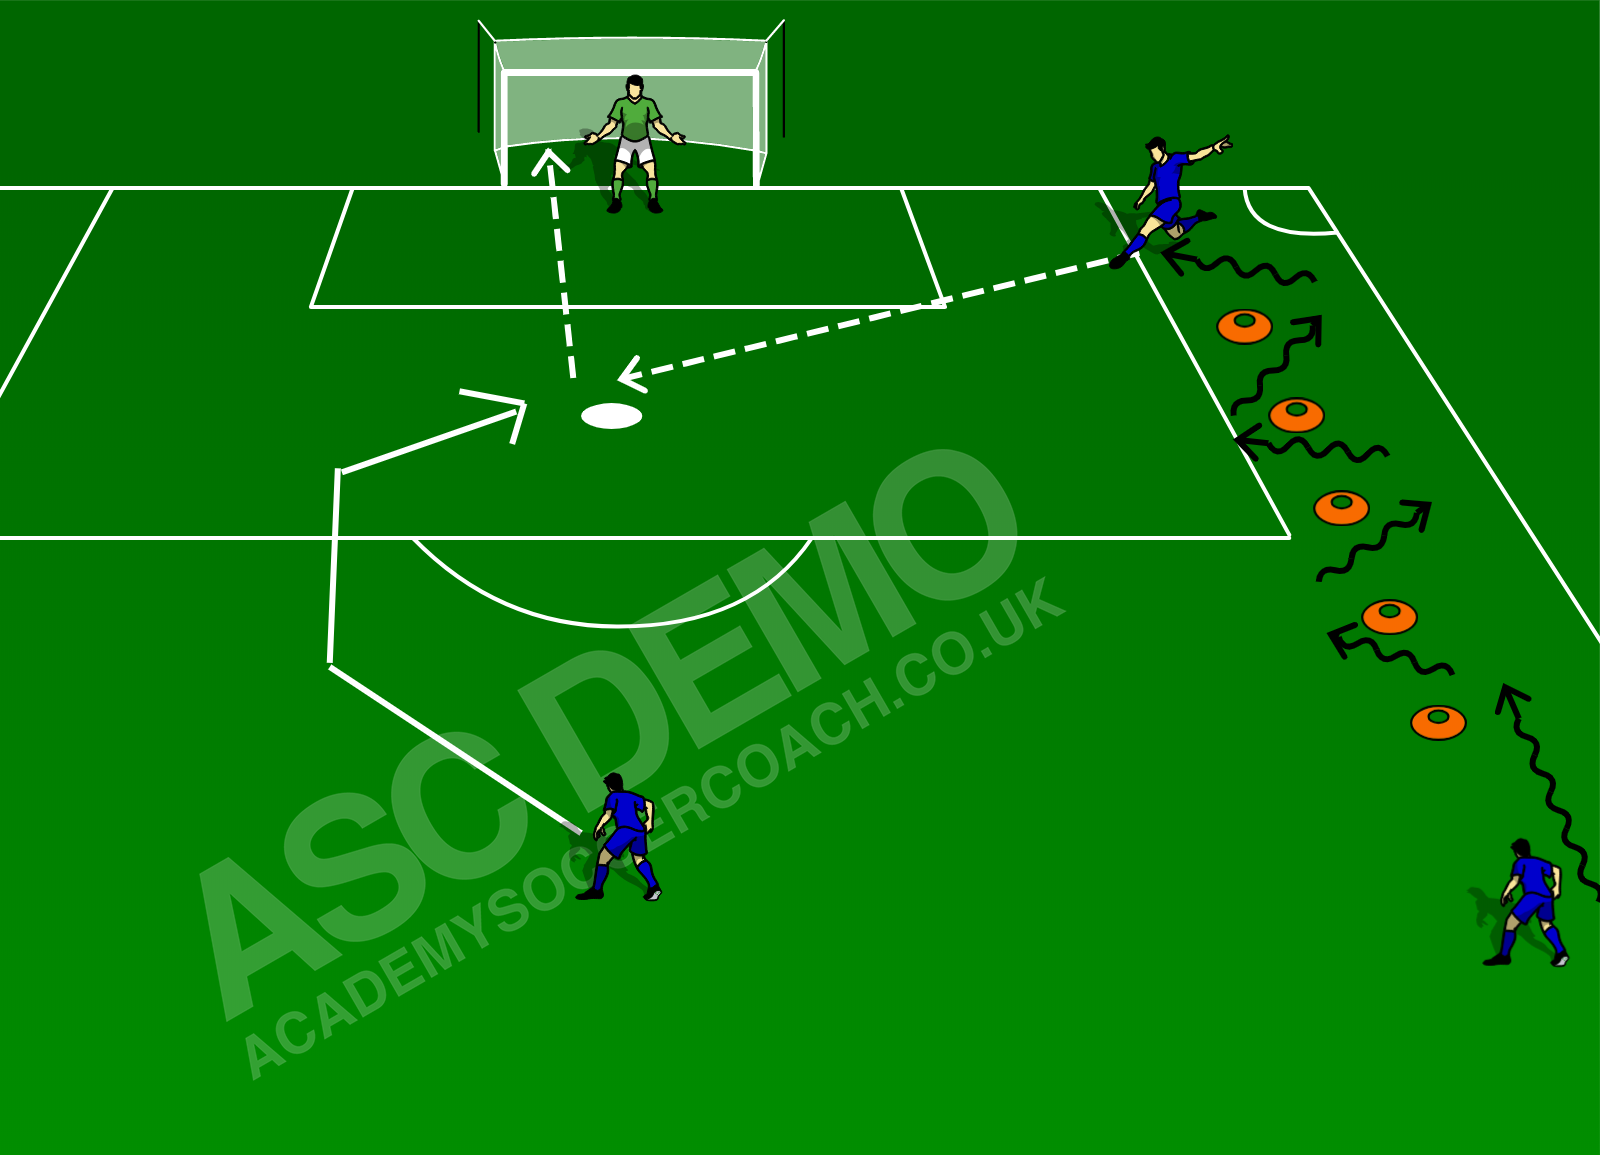
\includegraphics[width=\textwidth]{../img/Trimmed/Dribble-Cross-Shoot}
    \end{minipage}
    \hspace{0.05\linewidth}
    \begin{minipage}{.6\linewidth} % Left column and width
        \textbf{Drill Description:}
        \begin{enumerate}
        \setlength{\itemsep}{0pt}
        \setlength{\parskip}{0pt}
        \setlength{\parsep}{0pt}
        \item A line forms at half field, with a set of balls.
        \item Player 1 dribbles through cones, turning around the last cone toward goal,
        \item P1 then crosses the ball to the PK spot where the Striker takes his one touch shot.
        \item Striker retrieves the ball and goes to the end of the line.
        \item Wing then shifts to the striker role.
        \end{enumerate}

        \vspace{6pt}
        
        Once everyone goes once or twice switch side of the field and uses left feet for crossing and shooting.

        \vspace{6pt}
        
        Playing a Keeper is optional.

        \vspace{10pt}
        
        \textbf{Coaching Points:}
        \begin{itemize}
        \setlength{\itemsep}{0pt}
        \setlength{\parskip}{0pt}
        \setlength{\parsep}{0pt}
        \item The touch around that last cone is the most important. 
        \item Body position around that last cone is critical as well.  The players hips need to be tuned toward the PK spot otherwise the player gives up both power and control over the pass.
        \item The striker must be patient and not over run the spot.  Move in an arc away from center, then back toward the ball.  Accelerate once the ball is passed and kick it into goal.
        \end{itemize}

    \end{minipage}
\end{minipage}

\end{evenBlock}